\chapter{Anwendungen}
\label{cha:anwendungen}
% 6 Seiten

In den vergangen Jahren haben sich Unternehmen zunehmend an vielschichtigen neuronalen Netzen interessiert. Wie in Kapitel \ref{cha:entstehung} beschrieben, interessieren sich auch zunehmend Firmen wie Google, Apple und Microsoft. Sie stellten renommierte Wissenschaftler ein und kaufen Unternehmen die in diesem Bereich tätig sind.

\subsection{Objekterkennung in Bildern}

\begin{itemize}
\item 10 Millionen Trainingsbilder mit je 200x200 Pixel
\item Autoencoder mit sparse coding
\item 9 versteckte Schichten
\item 1 Milliarde Verbindungen
\item Training mit asynchronem stochastischem Gradientenvefahren
\item Auf auf 1000 Maschinen mit jeweils 16 Rechenkernen drei Tage lang trainiert
\end{itemize}

Bei einem Projekt \citep{googleimage} 2012 trainierte Google das bisher größte Netz dieser Art mit 10 Millionen Bilder aus dem Internet. Bekannt wurde das Projekt vor allem durch die Ausprägung des in Abbildung \ref{fig:neurons-google} zu sehenden Gesichts-, Katzen- und Körper-Neurons. Ein paar Eckdaten zum Netz und dem Training:

\begin{figure}%
\centering
\subfloat[menschliches Gesicht]{\begin{minipage}{0.33\textwidth}\centering%
	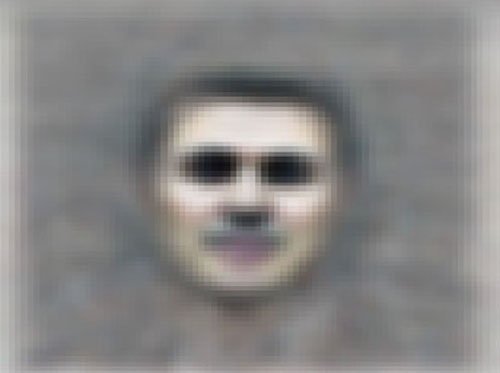
\includegraphics[width=0.9\textwidth]{images/neuron-face.jpg}\end{minipage}}
\subfloat[Gesicht einer Katze]{\begin{minipage}{0.33\textwidth}\centering%
	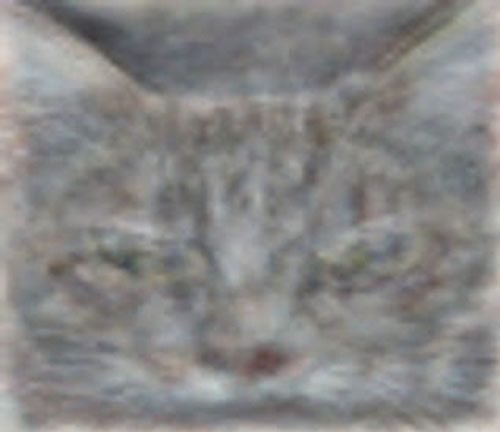
\includegraphics[width=0.9\textwidth]{images/neuron-cat.jpg}\end{minipage}}
\subfloat[menschlicher Körper]{\begin{minipage}{0.33\textwidth}\centering%
	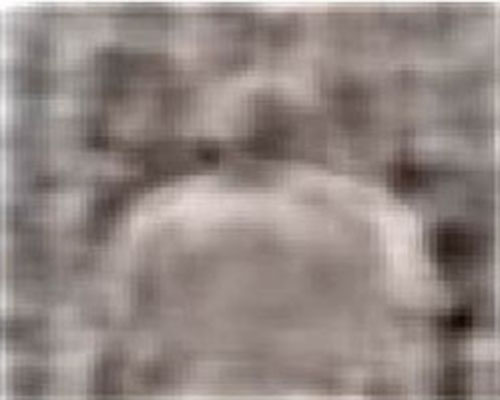
\includegraphics[width=0.9\textwidth]{images/neuron-body.jpg}\end{minipage}}
\caption{Markante Ausprägungen durch das lernen von Bildern aus dem Internet}
\label{fig:neurons-google}
\end{figure}

Es wurde mit relativ kleinen Bildern, dafür aber mit sehr vielen, unbeaufsichtigt trainiert. Ein späterer Benchmark auf ImageNET, eine Datenbank mit Kategorisierten Bildern, ergab einer Trefferquote von 15.8\%. Das entspricht einer Steigerung der bisherigen Bestleistung um 70\%.

Aus technischer Perspektive ist das Netz und damit die verwendete Technik weniger herausragend, als die Menge der Trainingsdaten und die damit verbunden Rechenleistung.

%google autoencoder, https://www.youtube.com/watch?v=g4ZmJJWR34Q  23:54
%36:00 L2 polling, ignoriert dass ein neuron invertiert ausgelößt wird, zählt alles + auch wenn negativ, da die welt/bilder auch immer verdreht und manipuliert daher kommt, sprache muss akzente ignorieren, gesichtserkennung die haarfarbet etc. auf der richtigen ebene an Features ist das daher ein sehr nützlicher faktor}
%\todo[inline]{local constrast normalization, hilft auch bilder invariationen zu ignorieren}
%\todo[inline]{google hat mit obrigen in den letzten jahren viel in der Bildersuche und youtube erreicht - was genau?, unsupervised learning mit einer unmänge an daten aus youtube videos}
%\todo[inline]{44:46+ bild: stages, drei stages mit jeweils in reihe: filtering, l2 polling, lcn (normalization step) - am ende haben einige neuronen muster erkannt, eines feuert bei gesichtern, eines bei katzen}
%\todo[inline]{49:02 number of parameters: 1 billion ... 200x200px bilder, 18x18 filters, 8 filters per location, l2 polling and lcn over 5x5 neighborhoods - wie viele neuronen gesamt?}
%\todo[inline]{wegen rechenpower nur mit sehr wenig pixel (200x200) gerechnet, unsere augen sehen n x n pixel, noch einiges möglich}
%\todo[inline]{the input image that maximises the neuron to fire: 53:00, das neuron war auf der 3. ebene} 
%\todo[inline]{neuron auf 1. ebene sind edges, 2. ebene kombinationen von edges, 3. ebene muster wie das gesicht}
%\todo[inline]{IMAGENET, Datenbank mit gelabelten bildern an der sich viele Benchmarken}
%erkennt kanten da farben von der beleuchtung abhängen und somit varriieren
%lernen mittels back propagation

\section{Zahlen erkennen

Google trainierte durch ihre Projekt Street View \citep{streetview} ein tiefes faltungskodiertes Netz, es lernte Hausnummern zu erkennen. Für die Adresssuche auf Google Maps und dem damit verbundenen Navigationssystem ist es von wesentlicher Bedeutung, Hausnummern richtig identifizieren zu können, besonders in den Gebieten, in denen Hausnummern nicht fortlaufend nummeriert sind.

Google trainierte mehrere Netze mit unterschiedlicher Anzahl an versteckten Schichten. Es stellte sich heraus, dass das tiefste Netz, mit elf versteckten Schichten, die Hausnummern am besten erkannte. Das Netz wurde mit über 100 Millionen hochauflösenden Bildern trainiert und forderte entsprechend viel Rechenleistung. Zum Training wurde der DistBelief-Alogrithmus \citep{distbelief} eingesetzt, ein Alogorithmus der sich besonders gut auf verteilt System berechnen lässt. 

Nummern die das Netz nicht auflösen konnte, haben unbewusst Menschen gelöst. Hierzu hat Google ein Projekt ins Leben gerufen, das Besucher von Webseiten an sicherheitsrelevanten Stellen einen Code identifizieren lässt um sicherzustellen dass es sich dabei tatsächlich um einen Menschen und keinen Bot handelt.

\begin{figure}
	\centering
	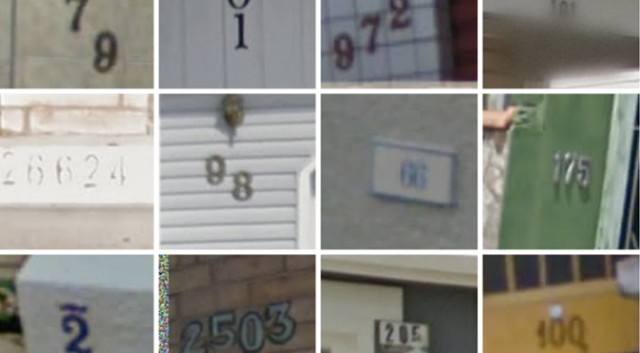
\includegraphics[width=0.7\textwidth]{images/streetview-numbers.jpg}
	\caption{Hausnummer die das neuronale Netz aus Google Street View erlernte.}
	\label{fig:streetview-numbers}
\end{figure}

Insgesamt hat das Netz bemerkenswert gut abgeschnitten \citep{numbercharts} und erkennt mittlerweile 97,84\% aller Hausnummern wie sie in Abbildung \ref{fig:streetview-numbers} zu sehen sind. Das Netz schaffte es sogar 99,8\% aller Sicherheitscodes der schwierigsten Art\footnote{http://www.google.com/recaptcha}, eingesetzt zum Schutz vor Bots auf Webseiten, zu lösen. Das Netz hat dabei besser als die meisten Menschen abgeschnitten, wodurch fraglich ist wie gut diese Sicherheitscodes in Zukunft tatsächlich vor Bots schützen werden.

\section{Spracherkennung}

Auch bei der Spracherkennung werden neuronale Netze in Kombination mit Deep Learning immer stärker und lösen nach und nach die Methode der Gaussian Mixture Models (GMM-Methoden) ab. Neuronale Netze für die Spracherkennung von Tonspuren funktionieren sehr ähnlich zu denen für die Bilderkennung. Wie bei der Bilderkennung prägen sich auf den ersten Schichten einfache Merkmale wie Konsonanten und Vokale aus. In höheren Schichten entstehen dann aussagekräftigere Merkmale bis hin zu vollständigen Wörtern, Phrasen und Stimmungen. 

Ein heute bereits verbreitetes Feld der Anwendung ist die Sprachsteuerung von Geräten, die quasi auf allen großen Plattformen\footnote{Google GOW Sprachsteuerung für Android-Geräte}\footnote{Apple Siri für IPhone-Geräte}\footnote{Microsoft Cortana für Windows Phone}\footnote{Diverse Systeme für Desktop-Betriebssysteme} verfügbar ist. Durch die große Menge an verfügbaren Sprachdaten von modernen Mobiltelefonen, die zudem sehr gut auf Personentypen deklariert werden können, ist zu erwarten, dass diese Netze in Zukunft noch stark an Bedeutung und Anwendungen gewinnen werden.

\section{Hardware}

2012 Hat Google mit einem neuronalen Netz, das drei Tage auf 1.000 Servern mit insgesamt 16.000 Rechenkernen lief, alles bisher dagewesen in den Schatten gestellt. Bereits 2013 Hat NVIDIA\todo{referenz} gemeinsam mit der Stanford Universität ein 6,5-fach größeres neuronales Netz auf GPUs realisiert. Das Netz benötigt lediglich 16 Computern mit jeweils vier Hochleistungs-Grafikkarten, die aber aus dem Konsumentenbereich stammen. Es ist also gelungen innerhalb von zwei Jahren Netze zu realisieren, die zuvor kaum möglich waren und dabei die Kosten für eine solche Implementierung weg von Supercomputern auf kleinere Servereinheiten bzw. Desktopcomputer holen.

Momentan entwickelt Qualcomm an Controller der eine relativ kleine neuronale Recheneinheit enthält. Der wesentliche Unterschied zu einer herkömmlichen CPU liegt dabei darin, dass alle Neuronen einer Schicht parallel rechnen. Das Netz benötigt daher nur wenige Zyklen bis zum Ergebnis, während herkömmliche CPUs jedes Neuron hintereinander berechnen müssen. In den frühen Entwicklungsstufen konnte das Netz bereits einige Bilderkennungsaufgaben ähnlich gut wie komplexe mathematische Algorithmen lösen. Der Chip soll 2014 in die Massenproduktion gehen und unter anderem in Mobiltelefonen zur Verfügung stehen.

\section{Weitere Anwendungen}

Weiter bemerkenswerte Anwendungsgebiete sind

\begin{itemize}
\item Erkennung von Verkehrsschildern, Benchmark bereits bei 99.91\% Trefferquote \citep{trafficsign}
\item Komprimierung von Daten
\item Alle Arten von Klassifizierungsaufgaben
\item Findung von Merkmalen in Daten
\end{itemize}

